\chapter{Unit Tests}
Dieses Kapitel befasst sich mit den Unit-Tests des Programmes. Dazu werden zuerst die ATRIP-Regeln erläutert und deren Anwendung beschrieben. Im Anschluss wird die Code Coverage erläutert. Zum Schluss wird noch auf die Verwendung von Mock-Objekten in den Unit-Tests eingegangen.

\section{ATRIP-Regeln}
Die ATRIP-Regeln sind Regeln, welche gute Unit-Tests einhalten sollten.
Die Regeln setzen sich wiefolgt zusammen:
\begin{itemize}
	\item Automatic - Eigenständig
	\item Thorough - Gründlich (genug)
	\item Repeatable - Wiederholbar
	\item Independent - Unabhängig voneinander
	\item Professional - Mit Sorgfalt hergestellt
\end{itemize}

\subsection{Automatic}
Die Regel \glqq{}Automatic\grqq{} besagt, dass die Tests ohne manuelle Eingriffe selbstständig ablaufen müssen. Weiterhin müssen die Tests auch ihre Ergebnisse selbst überprüfen. Als Ergebnisse sind dabei nur \glqq{}bestanden\grqq{} oder \glqq{}nicht bestanden\grqq{} zulässig. Durch die Anwendung dieser Regel ist es möglich Unit Tests zu automatisieren. \pagebreak

\lstinputlisting[
	label={code:automatic},
	caption={Automatic Unit Test},
	captionpos=b,
	style=EigenerJavaStyle
]{Quellcode/automatic.java}

In Quellcode \ref{code:automatic} ist ein Unit Test aus der Klasse BauerDienstTest zu sehen. In den Zeilen 14-16 überprüft der Test mithilfe von Assertions selbst sein Ergebnis. Das eigenstädnige ablaufen des Tests wird über Maven gewährleistet. Somit ist der Test Automatic.

\subsection{Thorough}
Die Regel \glqq{}Thorough\grqq{} besagt, dass alles Notwendige getestet werden muss. Die Definition von notwendig hängt dabei immer mit den Rahmenbedingungen zusammen. Mindestens muss aber jede missionskritische Funktionalität getestet werden und für jeden aufgetretenen Fehler muss ein Testfall existieren, welcher das erneute Auftreten des Fehlers verhindert. Durch diese Regel entstehen zusätzliche Tests im Umfeld von einem Fehler, um weitere Fehler zu verhindern.

Für den konkreten Fall des Schachspiels ist es notwendig jegliche Figuren-Dienste sowie den Kontrollierer für das Schachspiel zu testen. Daher sind für alle diese Klassen Unit Tests erstellt worden. Da es sich bei dem Programm um ein Spiel handelt, ist nahezu jede Funktion die Klassen missionskritisch. Da der Aufwand für jede Methode einen Unit Test zu programmieren zu hoch für dieses Projekt wäre, wurden zu jeder Klasse der Figuren-Dienste ein bis zwei Unit Tests implementiert.

\subsection{Repeatable}
Die Regel \glqq{}Repeatable\grqq{} besagt, dass jeder Test automatisch durchführbar sein sollte und dabei stets das gleiche Ergebnis liefern sollte. Dazu muss der Test unabhängig von der Umgebung sein. Dabei sind vor allem der Umgang mit einem Datum oder mit Zufallszahlen problematisch. Auch der Zugriff auf das Dateisystem stellt eine Abhängigkeit von der Umgebung dar.

Bei den implementierten Unit Tests gibt es keine Abhängigkeiten von der Umgebung. Die standardmäßigen Problemquellen sind für das Testen der Anwendung irrelevant, da weder Daten oder Zufallszahlen für das Testen des Schachspiels relevant sind noch ein Zugriff auf das Dateisystem in den Tests erfolgt. Das Spiel ist in sich selbst abgeschlossen, weshalb die Umgebung automatisch immer gleich ist.

\subsection{Independent}
Die Regel \glqq{}Repeatable\grqq{} besagt, dass Tests unabhängig von einander funktionieren müssen. Reihenfolge und Zusammenstellung müssen für ds ausführen der Tests irrelevant sein. Im Idealfall testet jeder Test genau einen Aspekt der zu testenden Komponente.

Da jeder Test alle benötigten Abhängigkeiten für sich selbst erzeugt erzeugt (mit zum Beispiel Mocks) gibt es keine Abhängigkeiten zu anderen Tests.

\subsection{Professional}
Die Regel \glqq{}Repeatable\grqq{} besagt, dass Testcode zum relevanten Produktionscode gehört und so leicht verständlich wie mögich sein sollte.

Um dies umzusetzen wurden zum einen sinnvolle Namen für die Testmethoden vergeben. So sind die Namen der Tests stets so aufgebaut, dass sie aus Methodenname + \glqq{}Test\grqq{} bestehen. Weiterhin sind die Tests an sich alle stets gleich aufgebaut. Zuerst werden die benötigten Abhängigkeiten erzeugt. Im Anschluss wird die zu testende Funktion ausgeführt und zum Schluss wird das Ergebnis überprüft. Durch diese Einheitliche Struktur wird für die Lesbarkeit der Tests gesorgt.  Weiterhin trägt auch eine simple Benennung von Variablen für gute Lesbarkeit.

\section{Code Coverage}
Die Code Coverage gibt an wie viel Quellcode mit Tests abgedeckt ist. Um die Code Coverage zu ermitteln kann eine Code Coverage Analyse in einer IDE ausgeführt werden. Bei Code Coverage unterschiedet man zwischen Line Coverage und Branch Coverage. Bei Line Coverage wird die Anzahl der getesten Zeilen des Quellcodes ins Verhältnis zur Gesamtzahl der Zeilen des Quellcodes gestellt. Branch Coverage hingegen beschreibt die Abdeckung von Verzweigungen im Code (if-statements). Wenn ein Test nur einen von zwei Pfaden abdeckt so liegt die Branch Coverage bei nur 50 Prozent. Bei der Code Coverage ist es wichtig dass stets angegeben wird, ob Line Coverage oder Branch Coverage verwendet wurde, da sich das Ergebnis dieser beiden Verfahren stark unterscheiden kann.

In Abbildung \ref{fig:CodeCoverage} sind die Ergebnisse einer Code Coverage Analyse für die Figuren-Dienste zu sehen. Dabei werden alle Klassen abgedeckt. Auch die Abdeckung der Methoden ist mit 94 Prozent sehr gut. Bei der Line Coverage kommen die Tests auf 59 Prozent und bei Branch Coverage nur auf 37 Prozent.
\begin{figure}[ht]
	\centering
	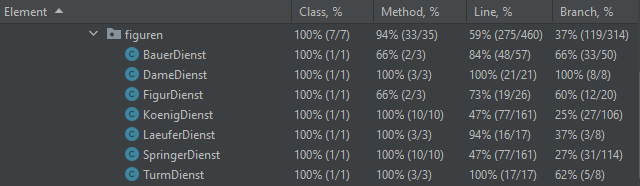
\includegraphics[width=0.8\textwidth]{Bilder/CodeCoverage.png} 
	\caption{Code Coverage-Analyse in IntelliJ für die Figuren-Dienste}
	\label{fig:CodeCoverage}
\end{figure}


\section{Mocks}
Als Mock-Objekte werden Stellvertreter für echte Objekte bezeichnet. Mithilfe dieser Stellvertreter können Abhängigkeiten bei der Durchführung von Tests ersetzt werden. Durch das ersetzen der Abhängigkeiten einer Klasse mit Mocks wird das isolierte Testen dieser Klasse möglich. Da es sehr aufwendig ist Mocks selber zu programmieren werden häufig Mock-Tools verwendet. Für den Einsatz eines Mocks muss das Mock-Objekt zuvor trainiert werden. Insgesamt durchläuft ein Mock-Objekt somit drei Phasen: Training-Phase, Einsatz-Phase und Verifikation-Phase. 

Für das Schachspiel wurde Mockito als Mock-Tool verwendet. Ein Beispiel für die Verwendung von Mocks ist in der Testklasse KoenigDienstTest zu sehen (siehe Quellcode \ref{code:Mocks} oder Github). 

\lstinputlisting[
	label={code:Mocks},
	caption={Verwendung von Mocks beim Testen},
	captionpos=b,
	style=EigenerJavaStyle
]{Quellcode/mocks.java}

In Quellcode \ref{code:Mocks} sind zwei Methoden aus der Klasse KoenigDienstTest zu sehen. Die Methode setUp (Zeile 1-8) wird vor jeder Testfunktion ausgeführt und initialisiert alle für die Tests benötigten Objekte. Unter diesen Objekten befindet sich neben einem KoenigDienst-Objekt und und einem Schachbrett-Objekt auch ein Mock-Objekt der Klasse Koenig. Das Mock-Objekt wird in Zeile 5 von Quellcode \ref{code:Mocks} erzeugt und in den Zeilen 6 und 7 eingelernt. In der Test-Methode getMoeglicheZuegeTest (Zeile 10-25 in Quellcode \ref{code:Mocks}) werden zunächst Testspezifische Mock-Objekte erzeugt. Da mit dieser Methode Interaktionen mit anderen Schachfiguren überprüft werden sollen, wird jeweils eine weiße und eine schwarze Dame als Mock-Objekt erzeugt (Zeile 12-13). In den Zeilen 14 bis 17 werden diese beiden Mock-Objekte eingelernt. Abgespielt werden die Mocks mit dem Funktionsaufruf \emph{koenigDienst.getMoeglicheZuege(figuren, schachbrett, koenigMock)} in Zeile 22. Im Anschluss wird überprüft, ob die angelernten Aufrufe mindestens ein mal genutzt wurden (Zeile 24 bis 31).